\documentclass[11pt]{article}
\usepackage{hyperref}
\usepackage{tabularx}
\usepackage{graphicx}
\usepackage{scalerel,stackengine}
\usepackage{adjustbox}
\usepackage{multirow}
\usepackage{ragged2e}
\stackMath
\newcommand\reallywidehat[1]{%
\savestack{\tmpbox}{\stretchto{%
  \scaleto{%
    \scalerel*[\widthof{\ensuremath{#1}}]{\kern-.6pt\bigwedge\kern-.6pt}%
    {\rule[-\textheight/2]{1ex}{\textheight}}%WIDTH-LIMITED BIG WEDGE
  }{\textheight}% 
}{0.5ex}}%
\stackon[1pt]{#1}{\tmpbox}%
}
\parskip 1ex
\graphicspath{ {./images/}}
%%%%%%%%%%%%%%%%%%%%%%%%%%%%%%%%%%%%%%%%%
% Lachaise Assignment
% Structure Specification File
% Version 1.0 (26/6/2018)
%
% This template originates from:
% http://www.LaTeXTemplates.com
%
% Authors:
% Marion Lachaise & François Févotte
% Vel (vel@LaTeXTemplates.com)
%
% License:
% CC BY-NC-SA 3.0 (http://creativecommons.org/licenses/by-nc-sa/3.0/)
% 
%%%%%%%%%%%%%%%%%%%%%%%%%%%%%%%%%%%%%%%%%

%----------------------------------------------------------------------------------------
%	PACKAGES AND OTHER DOCUMENT CONFIGURATIONS
%----------------------------------------------------------------------------------------

\usepackage{amsmath,amsfonts,stmaryrd,amssymb} % Math packages

\usepackage{enumerate} % Custom item numbers for enumerations

\usepackage[ruled]{algorithm2e} % Algorithms

\usepackage[framemethod=tikz]{mdframed} % Allows defining custom boxed/framed environments

\usepackage{listings} % File listings, with syntax highlighting
\lstset{
	basicstyle=\ttfamily, % Typeset listings in monospace font
}

%----------------------------------------------------------------------------------------
%	DOCUMENT MARGINS
%----------------------------------------------------------------------------------------

\usepackage{geometry} % Required for adjusting page dimensions and margins

\geometry{
	paper=a4paper, % Paper size, change to letterpaper for US letter size
	top=2.5cm, % Top margin
	bottom=3cm, % Bottom margin
	left=2.5cm, % Left margin
	right=2.5cm, % Right margin
	headheight=14pt, % Header height
	footskip=1.5cm, % Space from the bottom margin to the baseline of the footer
	headsep=1.2cm, % Space from the top margin to the baseline of the header
	%showframe, % Uncomment to show how the type block is set on the page
}

%----------------------------------------------------------------------------------------
%	FONTS
%----------------------------------------------------------------------------------------

\usepackage[utf8]{inputenc} % Required for inputting international characters
\usepackage[T1]{fontenc} % Output font encoding for international characters

\usepackage{XCharter} % Use the XCharter fonts

%----------------------------------------------------------------------------------------
%	COMMAND LINE ENVIRONMENT
%----------------------------------------------------------------------------------------

% Usage:
% \begin{commandline}
%	\begin{verbatim}
%		$ ls
%		
%		Applications	Desktop	...
%	\end{verbatim}
% \end{commandline}

\mdfdefinestyle{commandline}{
	leftmargin=pt,
	rightmargin=10pt,
	innerleftmargin=15pt,
	middlelinecolor=black!50!white,
	middlelinewidth=2pt,
	frametitlerule=false,
	backgroundcolor=black!5!white,
	frametitle={Command Line},
	frametitlefont={\normalfont\sffamily\color{white}\hspace{-1em}},
	frametitlebackgroundcolor=black!50!white,
	nobreak,
}

% Define a custom environment for command-line snapshots
\newenvironment{commandline}{
	\medskip
	\begin{mdframed}[style=commandline]
}{
	\end{mdframed}
	\medskip
}

%----------------------------------------------------------------------------------------
%	FILE CONTENTS ENVIRONMENT
%----------------------------------------------------------------------------------------

% Usage:
% \begin{file}[optional filename, defaults to "File"]
%	File contents, for example, with a listings environment
% \end{file}

\mdfdefinestyle{file}{
	innertopmargin=1.6\baselineskip,
	innerbottommargin=0.5\baselineskip,
	topline=false, bottomline=false,
	leftline=false, rightline=false,
	leftmargin=0cm,
	rightmargin=0cm,
	singleextra={%
		\draw[fill=black!10!white](P)++(0,-1.2em)rectangle(P-|O);
		\node[anchor=north west]
		at(P-|O){\ttfamily\mdfilename};
		%
		\def\l{3em}
		\draw(O-|P)++(-\l,0)--++(\l,\l)--(P)--(P-|O)--(O)--cycle;
		\draw(O-|P)++(-\l,0)--++(0,\l)--++(\l,0);
	},
	nobreak,
}

% Define a custom environment for file contents
\newenvironment{file}[1][File]{ % Set the default filename to "File"
	\medskip
	\newcommand{\mdfilename}{#1}
	\begin{mdframed}[style=file]
}{
	\end{mdframed}
	\medskip
}

%----------------------------------------------------------------------------------------
%	NUMBERED QUESTIONS ENVIRONMENT
%----------------------------------------------------------------------------------------

% Usage:
% \begin{question}[optional title]
%	Question contents
% \end{question}

\mdfdefinestyle{question}{
	innertopmargin=1.2\baselineskip,
	innerbottommargin=0.8\baselineskip,
	roundcorner=5pt,
	nobreak,
	singleextra={%
		\draw(P-|O)node[xshift=1em,anchor=west,fill=white,draw,rounded corners=5pt]{%
		Question \theQuestion\questionTitle};
	},
}

\newcounter{Question} % Stores the current question number that gets iterated with each new question

% Define a custom environment for numbered questions
\newenvironment{question}[1][\unskip]{
	\bigskip
	\stepcounter{Question}
	\newcommand{\questionTitle}{~#1}
	\begin{mdframed}[style=question]
}{
	\end{mdframed}
	\medskip
}

%----------------------------------------------------------------------------------------
%	WARNING TEXT ENVIRONMENT
%----------------------------------------------------------------------------------------

% Usage:
% \begin{warn}[optional title, defaults to "Warning:"]
%	Contents
% \end{warn}

\mdfdefinestyle{warning}{
	topline=false, bottomline=false,
	leftline=false, rightline=false,
	nobreak,
	singleextra={%
		\draw(P-|O)++(-0.5em,0)node(tmp1){};
		\draw(P-|O)++(0.5em,0)node(tmp2){};
		\fill[black,rotate around={45:(P-|O)}](tmp1)rectangle(tmp2);
		\node at(P-|O){\color{white}\scriptsize\bf !};
		\draw[very thick](P-|O)++(0,-1em)--(O);%--(O-|P);
	}
}

% Define a custom environment for warning text
\newenvironment{warn}[1][Warning:]{ % Set the default warning to "Warning:"
	\medskip
	\begin{mdframed}[style=warning]
		\noindent{\textbf{#1}}
}{
	\end{mdframed}
}

%----------------------------------------------------------------------------------------
%	INFORMATION ENVIRONMENT
%----------------------------------------------------------------------------------------

% Usage:
% \begin{info}[optional title, defaults to "Info:"]
% 	contents
% 	\end{info}

\mdfdefinestyle{info}{%
	topline=false, bottomline=false,
	leftline=false, rightline=false,
	nobreak,
	singleextra={%
		\fill[black](P-|O)circle[radius=0.4em];
		\node at(P-|O){\color{white}\scriptsize\bf i};
		\draw[very thick](P-|O)++(0,-0.8em)--(O);%--(O-|P);
	}
}

% Define a custom environment for information
\newenvironment{info}[1][Info:]{ % Set the default title to "Info:"
	\medskip
	\begin{mdframed}[style=info]
		\noindent{\textbf{#1}}
}{
	\end{mdframed}
}
 

\title{AMS 578 Spring 2021\\Multiple Regression Computing Project\\Final Report}

\author{
  Kai Li\thanks{Department of Applied Mathematics and Statistics, Stony Brook University, email: \href{mailto:kai.li@stonybrook.edu}{kai.li@stonybrook.edu}}
}

\date{Stony Brook University --- \today}

\begin{document}
\maketitle

\section{Introduction}
Depression is one of the top five leading causes of disability and disease burden worldwide \cite{ar:caspi}. Researchers such as Caspi et al. \cite{ar:caspi} and Risch et al. \cite{ar:risch} have already conducted meta-analyses of the interaction between the serotonin transporter gene (5-HTTLPR) and stressful life events on the risk of depression using regression techniques. This multiple regression computing project aims to analyze a given synthetic dataset to fit a model using statistical software \texttt{R} given the background of related studies.

There are a few steps to perform a complete regression analysis. The first step is data summarizing and cleaning. Then, since variables can be nonlinear, checking if transformations are required is a key to ensure proper analysis and conclusion. An examination of important independent variables for the model becomes the following procedure. Especially, given a lack of consensus from the background, gene-by-environment and gene-by-gene interaction require additional inspection \cite{ar:caspi, ar:risch}. It is also given that at most four-way interactions of independent variables will appear. Finally, compare and determine if regression results are viable.

The preliminary report shows the summary statistics table for the given dataset, the methodology used to deal with the missing data, and a close inspection of multicollinearity of the complete imputed datasets. The final report is a continuation of the preliminary report, which investigates regression model assumptions, the candidate regressors added in the model, model selection, analyses of candidate regression models, and pooling of parameters. The final report is divided into methods, results, conclusions and discussion, and appendix sections.

\section{Methods}
After summarizing and cleaning data, it is essential to check assumptions for linear regression. Before that, recall from the preliminary report that the methodology used to cope with the missing values in the original dataset is the multiple imputation technique. To generate unbiased estimates and correct confidence intervals utilizing this method, analyses of the two imputed datasets individually before pooling the parameters are necessary \cite{bk:buuren, ar:raghunathan}. Therefore, assumption verifications should be done for both imputed datasets, similarly for other applied linear regression analysis procedures, such as variable selection.

Kutner et al. \cite{bk:kutner} and Montgomery et al. \cite{bk:montgomery} generalize the following major assumptions in linear regression theory:
\begin{enumerate}
\item The relationship between the dependent and independent variables should be at least approximately linear.
\item The error term has zero mean.
\item The error term has constant variance.
\item The errors are uncorrelated.
\item The errors follow a normal distribution.
\end{enumerate}
Residual plots, including residuals vs. fitted, normal Q-Q (normal probability), scale-location, and residuals vs. leverage plots, can help inspect the assumptions and detect model inadequacies \cite{bk:kutner, bk:montgomery}. In practice, Kutner et al. \cite{bk:kutner} and Montgomery et al. \cite{bk:montgomery} suggest performing residual analysis of every regression model to ensure model adequacy, including the models obtained from transformations and stepwise regression procedures. If there are issues with nonlinearity, distribution of error terms, and unequal error variances, transformations of the dependent variable and independent variables are the appropriate next steps \cite{bk:kutner}. In particular, data transformation enables response and regressors to be in the correct scale or unit of measurement, where violations of the five basic regression assumptions are no longer exist \cite{bk:montgomery}. Several techniques provide guidelines on fixing the issue of assumption violations, such as variance stabilizing, model linearization, and nonnormality correction. In this paper, transformations in the response variable will first be considered. Then, residual analysis on the transformed imputed datasets will be conducted to see if the underlying assumptions are met. If not, additional transformations on the regressor variables will be considered, again performing residual analysis after that. Also, transformations to linearize the regression model can be attempted if transformations on the dependent variable are insufficient.

When all the assumptions are satisfied for both datasets, exploring the candidate independent variables and their interaction terms in the model follows. It is essential to keep the order of the regression model as low as possible \cite{bk:kutner, bk:montgomery}. Variable selection based on stepwise regression procedures will first be performed for the two imputed datasets. After that, fit linear regression models on those regressors with eight criteria examining the candidate models: $\textrm{SSE}_p$, $\textrm{MSE}_p$, $R_p^2$, $R_{a, p}^2$, $\textrm{AIC}_p$, $\textrm{BIC}_p$, $\textrm{PRESS}_p$, and $\textrm{max(VIF)}$. Next, it is appropriate to inspect several related possible regression models provided the insights on the subject area for this project and additional candidate variables selected, such as interaction terms. The first trivial model for a dataset concerns the regression with the intercept only. Then, candidate variables without interaction terms are fitted to evaluate their appropriateness. After that, given that at most four-way interaction terms present, high-order interactions will be fitted to observe if the interaction terms are significant in stepwise procedures. All candidate models will be assessed and compared by the eight criteria. This part corresponds to the first part of model adequacy verification, using well-developed criterion. The most preferred candidate model for each imputed dataset will be determined.

The second part of model adequacy checking verifies the candidate models' assumptions and inspects influential and high-leverage observations. Unsurprisingly, residual plots are still the most powerful tools. Analysis of Variance (ANOVA) inspects the overall and individual effects of regressors in a model compared to the intercept-only model. If the regressors are significant and residual plots indicate an expected pattern, the model adequacy to the goal and the background for the project will be validated to reach the objective for this project. Finally, pooling of the parameters from the two candidate models will be done to output the final fitted model.

\section{Results}
First, assumptions of linear regression for both imputed datasets are verified. Both imputed datasets violate some of the linear regression assumptions, but the patterns of the residual plots are very similar. The residual vs. fitted values plots of the datasets indicate a violation of linearity and independence assumptions. The homoscedasticity assumption is violated by inspecting the scale-location plots. Based on the normal Q-Q plots, it is reasonable to have the normality assumption for both datasets. Hence, transformations are required for both imputed datasets to continue with multiple linear regression procedures.

The first transformation procedure considers transforming the response variable. Box-Cox transformations are used here. For both imputed datasets, the parameter $\lambda$ obtained using the Box-Cox method returns value 0. In other words, if $y$ is denoted to be the dependent variable values, then the transformations are $y'=\ln{y}$ for the two imputed datasets. By examining the residuals vs. fitted plots, normal Q-Q plots, and scale-location plots for both transformed datasets again, the transformations provide a satisfactory solution to handle assumption violations of the imputed datasets. That is, for both datasets, the relationship between the dependent and independent variables is approximately linear; the error term has a mean close to 0 and approximately constant variance; the errors can be assumed to be uncorrelated; the errors are normally distributed. Hence, the five basic regression assumptions are considered met after transforming the response.

Based on the analysis of the residual plots, a first-order regression model is sufficient and appropriate for both datasets. Stepwise regression is ready to run. \autoref{tab:model} shows the selected possible regression models and the eight criteria statistics based on the stepwise regression procedures and insights given the background of the original dataset. It is crucial to remark that the stepwise regression candidate variable outputs are the same for both imputed datasets. Also, the statistics obtained from the eight criteria are very similar. Therefore, the conclusion for the model selection process should be the same. The report will mainly discuss detailed results for the first imputed dataset.

\begin{table}[ht]
\centering
\begingroup
\caption{$\textrm{SSE}_p$, $\textrm{MSE}_p$, $R_p^2$, $R_{a, p}^2$, $\textrm{AIC}_p$, $\textrm{BIC}_p$, $\textrm{PRESS}_p$, and $\textrm{max(VIF)}$ Values for Selected Possible Regression Models for the First Imputed Dataset} 
\label{tab:model}
\begin{adjustbox}{width=\textwidth}
\begin{tabular}{llllllllll}
\hline
$\mathbf{X}$ & \textbf{(1)} & \textbf{(2)} & \textbf{(3)} & \textbf{(4)} & \textbf{(5)} & \textbf{(6)} & \textbf{(7)} & \textbf{(8)} & \textbf{(9)} \\
\textbf{Variables} & \multirow{2}{*}{$\mathbf{p}$} & \multirow{2}{*}{$\mathbf{SSE_p}$} & \multirow{2}{*}{$\textbf{MSE}_p$} & \multirow{2}{*}{$\mathbf{R_p^2}$} & \multirow{2}{*}{$\mathbf{R_{a, p}^2}$} & \multirow{2}{*}{$\mathbf{AIC_p}$} & \multirow{2}{*}{$\mathbf{BIC_p}$} & \multirow{2}{*}{$\mathbf{PRESS_p}$} & \textbf{max} \\
\textbf{in Model} &  &  &  &  &  &  &  &  & \textbf{(VIF)} \\ 
  \hline
None & $\mathsf{1}$ & $\mathsf{110.6}$ & $\mathsf{0.060}$ & $\mathsf{0.000}$ & $\mathsf{0.000}$ & $\mathsf{44.60}$ & $\mathsf{55.65}$ & $\mathsf{4.4\times10^{23}}$ & NA \\

\\

E4, E5, R1, R7, R16 & $\mathsf{6}$ & $\mathsf{69.76}$ & $\mathsf{0.038}$ & $\mathsf{0.369}$ & $\mathsf{0.368}$ & $\mathsf{-797.1}$ & $\mathsf{-758.4}$ & $\mathsf{4.4\times10^{23}}$ & $\mathsf{1.003}$ \\

\\

E4, E5, R1, R7, R16 & \multirow{3}{*}{$\mathsf{9}$} & \multirow{3}{*}{$\mathsf{47.38}$} & \multirow{3}{*}{$\mathsf{0.026}$} & \multirow{3}{*}{$\mathsf{0.572}$} & \multirow{3}{*}{$\mathsf{0.570}$} & \multirow{3}{*}{$\mathsf{-1506}$} & \multirow{3}{*}{$\mathsf{-1451}$} & \multirow{3}{*}{$\mathsf{4.4\times10^{23}}$} & \multirow{3}{*}{$\mathsf{3.091}$} \\
R1$\times$R7, R1$\times$R16,  &  &  &  &  &  &  &  &  & \\
R7$\times$R16 &  &  &  &  &  &  &  &  & \\

\\

E4, E5, R1, R7, R16 & \multirow{3}{*}{$\mathsf{10}$} & \multirow{3}{*}{$\mathsf{46.73}$} & \multirow{3}{*}{$\mathsf{0.025}$} & \multirow{3}{*}{$\mathsf{0.577}$} & \multirow{3}{*}{$\mathsf{0.575}$} & \multirow{3}{*}{$\mathsf{-1529}$} & \multirow{3}{*}{$\mathsf{-1469}$} & \multirow{3}{*}{$\mathsf{4.4\times10^{23}}$} & \multirow{3}{*}{$\mathsf{38.55}$} \\
R1$\times$R7, R1$\times$R16, &  &  &  &  &  &  &  &  & \\
R7$\times$R16, E4$\times$E5 &  &  &  &  &  &  &  &  & \\

\\

E4, E5, R1, R7, R16 & \multirow{3}{*}{$\mathsf{10}$} & \multirow{3}{*}{$\mathsf{42.05}$} & \multirow{3}{*}{$\mathsf{0.023}$} & \multirow{3}{*}{$\mathsf{0.620}$} & \multirow{3}{*}{$\mathsf{0.618}$} & \multirow{3}{*}{$\mathsf{-1724}$} & \multirow{3}{*}{$\mathsf{-1664}$} & \multirow{3}{*}{$\mathsf{4.4\times10^{23}}$} & \multirow{3}{*}{$\mathsf{7.259}$} \\
R1$\times$R7, R1$\times$R16, &  &  &  &  &  &  &  &  & \\
R7$\times$R16, R1$\times$R7$\times$R16 &  &  &  &  &  &  &  &  & \\
  \hline
\end{tabular}
\end{adjustbox}
\endgroup
\footnotesize
\end{table}

Note that interactions between the environment candidate variables and the gene candidate variables are not significant and therefore not considered the candidates of regressors. Moreover, the four-way interaction of candidate gene variables is not significant and thus omitted as well. The fourth model with an environment-by-environment interaction term yields a significant multicollinearity problem among the five selected models. Hence, any model with an environment-by-environment interaction is excluded. Also, notice that the fifth model with a three-way interaction term of candidate gene variables has a potential multicollinearity issue as well, depending on the threshold of potential multicollinearity. The preliminary report suggests a multicollinearity issue for a maximum of VIF greater than 10 \cite{bk:kutner}. Montgomery et al. \cite{bk:montgomery} recommend that a VIF greater than 5 or 10 suggests the problem with potential multicollinearity. Given that other criteria do not deviate much, the three-way-interaction model will be excluded due to robustness and simplicity. After that, by comparing and analyzing the interpretation of the criterion of the top three models, the third candidate model with three one-way interactions is selected as the preferred candidate model for now. The same decision applies to the second imputed dataset.

Before concluding the models to be the final fits for the two imputed datasets, it is important to confirm the regressors are significant in the fitted candidate models through ANOVA. In particular, the first step is to inspect whether the joint effect of all regressors is significant. The ANOVA statistics for the first imputed dataset are shown in \autoref{tab:anova1}.

\begin{table}[ht]
\centering
\begingroup\footnotesize
\caption{Analysis of Variance for Significance of Joint Regression for the First Imputed Dataset} 
\label{tab:anova1}
\begin{adjustbox}{width=\textwidth}
\begin{tabular}{lccccc}
\hline
\textbf{Source of Variation} & \textbf{Sum of Squares} & \textbf{Degrees of Freedom} & \textbf{Mean Square} & $\mathrm{F}_0$ & \textbf{P-Value} \\ 
\hline
Regression & $\mathsf{63.225}$ & $\mathsf{8}$ & $\mathsf{7.903}$ & $\mathsf{306.75}$ & $\mathsf{< 2.2\times 10^{-16}}$ \\
Residual & $\mathsf{47.379}$ & $\mathsf{1839}$ & $\mathsf{0.026}$ &  &  \\
Total & $\mathsf{110.60}$ & $\mathsf{1847}$ &  &  &  \\
\hline
\end{tabular}
\end{adjustbox}
\endgroup
\end{table}

The P-value is very small, suggesting that the log of the dependent variable is related to at least one of the candidate regressors. Thus, at least one of the regressors is important, meaning that the candidate independent variables in the candidate model improve the fit. The conclusion is the same for the second imputed dataset. A logical question next becomes which one(s) are crucial. The results for hypothesis testing of the individual regressor effect are shown in \autoref{tab:anova2}.

\begin{table}[ht]
\centering
\begingroup\footnotesize
\caption{Analysis of Variance for Significance of Individual Regression for the First Imputed Dataset} 
\label{tab:anova2}
\begin{adjustbox}{width=\textwidth}
\begin{tabular}{lccccc}
\hline
\textbf{Source of Variation} & \textbf{Sum of Squares} & \textbf{Degrees of Freedom} & \textbf{Mean Square} & $\mathrm{F}_0$ & \textbf{P-Value} \\ 
\hline
E4 & $\mathsf{15.93}$ & $\mathsf{1}$ & $\mathsf{15.93}$ & $\mathsf{618.16}$ & $\mathsf{< 2.2\times 10^{-16}}$ \\
E5 & $\mathsf{5.909}$ & $\mathsf{1}$ & $\mathsf{5.909}$ & $\mathsf{229.37}$ & $\mathsf{< 2.2\times 10^{-16}}$ \\
R1 & $\mathsf{8.192}$ & $\mathsf{1}$ & $\mathsf{8.192}$ & $\mathsf{317.96}$ & $\mathsf{< 2.2\times 10^{-16}}$ \\
R7 & $\mathsf{5.503}$ & $\mathsf{1}$ & $\mathsf{5.503}$ & $\mathsf{213.60}$ & $\mathsf{< 2.2\times 10^{-16}}$ \\
R16 & $\mathsf{5.311}$ & $\mathsf{1}$ & $\mathsf{5.311}$ & $\mathsf{206.16}$ & $\mathsf{< 2.2\times 10^{-16}}$ \\
R1$\times$R7 & $\mathsf{6.732}$ & $\mathsf{1}$ & $\mathsf{6.732}$ & $\mathsf{261.28}$ & $\mathsf{< 2.2\times 10^{-16}}$ \\
R1$\times$R16 & $\mathsf{9.095}$ & $\mathsf{1}$ & $\mathsf{9.095}$ & $\mathsf{353.00}$ & $\mathsf{< 2.2\times 10^{-16}}$ \\
R7$\times$R16 & $\mathsf{6.557}$ & $\mathsf{1}$ & $\mathsf{6.557}$ & $\mathsf{254.50}$ & $\mathsf{< 2.2\times 10^{-16}}$ \\
Residual & $\mathsf{47.379}$ & $\mathsf{1839}$ & $\mathsf{0.026}$ &  &  \\
Total & $\mathsf{110.60}$ & $\mathsf{1847}$ &  &  &  \\
\hline
\end{tabular}
\end{adjustbox}
\endgroup
\end{table}

The P-values of all the candidate regressors are small, meaning that the candidate variables are all significant. Thus, including every candidate regressor can improve the fit for the first imputed data, and the same conclusion can be drawn for the second imputed dataset.

For model adequacy checking and validation, the residuals vs. fitted plot \autoref{fig:residuals} provides a satisfactory output because the red line is satisfactorily straight except for the boundary where some underlying influential points present. Expectedly, the normal probability and scale-location plots behave naturally, and therefore the elementary assumptions are not considered violated in the candidate model for the first imputed dataset, similarly for the second.

\begin{figure}[h!]
\begin{center}
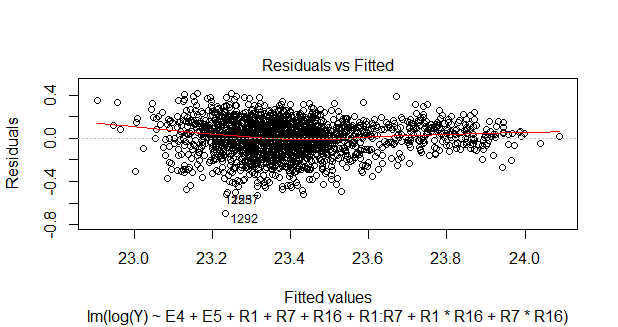
\includegraphics[scale=0.69]{residuals}
\end{center}
\caption{Residuals vs. Fitted Plot}
\label{fig:residuals}
\end{figure}

The extreme values have to be investigated as well. The points can be leverage or influential observations. \autoref{fig:leverage} is a residuals vs. leverage plot that depicts Cook's distances comparing fit. From the plot, several leverage observations exist, but most data points behave naturally in a cluster. Moreover, only a few points have high Cook’s distance scores compared to a large number of observations. Thus, the extreme points will not drastically affect the coefficients of the candidate regressors for the first imputed dataset. The second imputed dataset candidate model yields a similar residuals vs. leverage plot as the first imputed dataset. 

\begin{figure}[h!]
\begin{center}
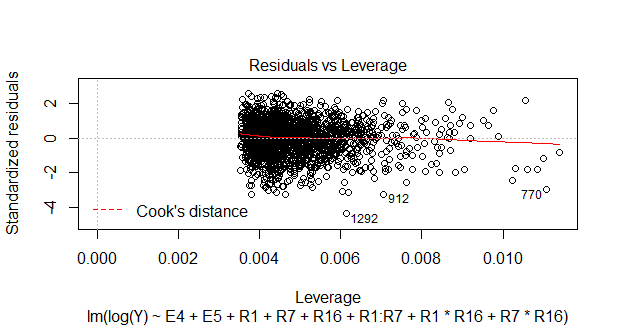
\includegraphics[scale=0.69]{leverage}
\end{center}
\caption{Residuals vs. Leverage Plot}
\label{fig:leverage}
\end{figure}

Finally, model validation requires an analysis of whether the model will function successfully in the given background. Research conducted by Caspi et al. \cite{ar:caspi} and Risch et al. \cite{ar:risch} illustrated the relationship between life stress events and the risk of depression, with polymorphism in the 5-HTTLTR serotonin transporter gene moderating the influence of the relationship. Here, the quantitative measurement of depression is the response variable \texttt{Y}; \texttt{E} represents the quantitative measurement of different life stress events; \texttt{R} consists of indicator variables denoting specific genes. The Risch et al. \cite{ar:risch} meta-analysis results demonstrated a potential relationship between stressful life events and the risk of depression. In the candidate model, the effect of the environment on depression is significant, though the interaction between environment candidate variables is excluded from multicollinearity. Moreover, the interaction terms between \texttt{E} and \texttt{R} are all not significant, and therefore not appeared in the candidate models. However, three lines of experimental research reported a gene-by-environment interaction \cite{ar:caspi}. Also, Caspi et al. \cite{ar:caspi} showed a significant interaction between the environment candidate variables and the gene candidate variables. On the other hand, Risch et al. \cite{ar:risch} claimed no evidence of the interaction between \texttt{E} and \texttt{R}, also shown in other meta-analyses studies in Risch et al.'s \cite{ar:risch} paper. Due to limitations of meta-analysis, the research framework of Caspi et al. \cite{ar:caspi} may have led to different findings compared to the originally reported findings, which may result in a false positive report \cite{ar:risch}. What is more, Caspi et al. \cite{ar:caspi} suggested the possibility of misidentifying a gene-by-environment interaction but, in fact, a gene-by-gene interaction. In this project, interactions between gene candidate variables are significant. A valid confirmation of Caspi et al. \cite{ar:caspi} results is needed \cite{ar:risch}. Hence, the candidate model's lack of gene-by-environment interactions and the presence of gene-by-gene interactions are plausible and appropriate for the project. To summarize, the candidate model is validated with enough supportive research evidence. 

Last but not least, the final model for the original dataset can be obtained by pooling the parameters using multiple imputation techniques. The model is shown in \autoref{eq:model}. 

\begin{multline}\label{eq:model}
\ln{\hat{\textrm{Y}}}=\,22.857+0.000571\,\textrm{E4}+0.000330\,\textrm{E5}-0.1353\,\textrm{R1}-0.1384\,\textrm{R7}-0.1515\,\textrm{R16}\\
+0.2500\,\textrm{R1$\times$R7}+0.2732\,\textrm{R1$\times$R16}+0.2398\,\textrm{R7$\times$R16}.
\end{multline}

\section{Conclusions and Discussion}
The project aims at finding an appropriate linear regression model for a given synthetic dataset with related background studies. The research started with summarizing and cleaning datasets so that a general understanding of the data is acquired. Multiple imputation was used to compensate for the missing information from the original data. Then, analysis on assumptions verification and transformation procedures for imputed datasets enabled to perform an unbiased and correct regression. The best candidate model for each imputed dataset was evaluated and chosen by the eight criteria and residual plots through a series of attempts on fitting candidate models with candidate variables selected from stepwise regression. Next, the candidate models chosen were verified viable because they matched the expectations given from the mental illness subject background. Finally, the model for this project was selected through parameters pooling.

There are certain limitations and weaknesses in this project. First, since the synthetic dataset is observational, the given dataset and the final model do not provide adequate information about cause-and-effect relationships \cite{bk:kutner, bk:montgomery}. Moreover, since multiple imputation is not an easy technical fix for the missing values in a dataset, extra caution is needed so that the likelihood of getting nonsensible or even misleading results is small \cite{bk:buuren}. Especially, Buuren \cite{bk:buuren} clarifies the danger of solely using computer software to obtain outputs for using multiple imputation. Furthermore, VIF cannot distinguish between several simultaneous multicollinearities, which means additional care and insight to detect multicollinearity is needed \cite{bk:kutner, bk:montgomery}. Thus, the nature of the multicollinearity may not be identified. Additionally, residual plots may not correctly show the nature behind the marginal effect, given the other regressors in the model \cite{bk:kutner}. A more sophisticated method called partial regression plots or added-variable plots can identify the marginal effects in a regression model \cite{bk:kutner, bk:montgomery}. Regardless, the final model obtained in this report is still meaningful and satisfactory.

\appendix
\section{Technical Implementation in \texttt{R}}
Because multiple imputation technique, with two imputed datasets outputted, is used, each dataset should be inspected and analyzed on its own before pooling the parameters across the two analyses \cite{bk:buuren}. The technical implementations in \texttt{R} for the procedures in the two imputed datasets are identical except for changing all \texttt{data1} to \texttt{data2} in the code. Therefore, the implementation details for the second imputed dataset are omitted.

\subsection{Regression Analysis Assumptions Verification}
The validity of regression analysis assumptions should always be examined  by inspecting the adequacy of the tentative model \cite{bk:montgomery}. Residual plots are powerful tools for detecting violations of the five basic regression assumptions \cite{bk:montgomery}. In \texttt{R}, function \texttt{plot()} outputs the four plots for a given linear regression \texttt{lm()}, which provide tremendous help in examining the assumptions. Readability can be enhanced if function \texttt{par()} is utilized to arrange the four plots in two rows and two columns.

\begin{file}[project.r]
\begin{lstlisting}[language = R]
fit1 <- lm(Y ~ ., data = data1)
par(mfrow = c(2, 2))
plot(fit1)
\end{lstlisting}
\end{file}

The residuals vs. fitted plot indicates the need for a curvilinear regression function, which means the presence of nonlinearity \cite{bk:kutner, bk:montgomery}. Moreover, the zero error mean assumption can be assumed given that the intercept term is added to the model. The scale-location plot can check the constancy of the error variance. The curvilinear red line indicates a possibly nonconstant variance. Furthermore, the uncorrelated error assumption can be checked in a method similar to the checking linearity assumption. In other words, the nonstraight red line shows a possible correlation between the error terms. Finally, the normal Q-Q plot indicates a satisfactory deviation from the normal line. Thus, it is reasonable to assume that the errors are normally distributed.

\subsection{Box-Cox Transformations}
Box-Cox transformations are useful in transforming the dependent variable to correct nonnormality or nonconstant variance. In particular, The Box-Cox procedure uses the method of maximum likelihood (ML) to estimate the parameter $\lambda$ \cite{bk:kutner}. In the \texttt{MASS} package, \texttt{boxcox()} computes the log-likelihood given $\lambda$ values from -2 to 2 in steps of 0.1 by default. In the following implementation, \texttt{x} represents $\lambda$ values, and \texttt{y} represents the log-likelihood values in the output of the function \texttt{boxcox()}.

\begin{file}[project.r]
\begin{lstlisting}[language = R]
library(MASS)
bc1 <- boxcox(Y ~ ., data = data1, plotit = FALSE)
lambda1 <- bc1$x[which.max(bc1$y)]
\end{lstlisting}
\end{file}
The $\lambda$ value returned by the Box-Cox method is 0 for both imputed datasets, corresponding to the transformations that $y'=\ln{y}$ in the response. Then, it is crucial to inspect whether a violation of assumptions exists after the transformations.

\begin{file}[project.r]
\begin{lstlisting}[language = R]
fit2 <- lm(log(Y) ~ ., data = data1)
plot(fit2)
\end{lstlisting}
\end{file}

Residual analyses for both imputed datasets provide the same conclusion. The residuals vs. fitted plot shows a far less curvilinear line. The line is almost straight, which gives a satisfactory transformation in terms of linearity and correlation of the errors. The scale-location plot also suggests a significant improvement in stabilizing the variance of both datasets. The error term has zero mean assumption is assumed because the model has an intercept term. Visually speaking, though the normal probability plot already illustrates the normality without transformations, the datasets fit the normal line more perfectly after the transformations. To conclude, the transformations are effective.

\subsection{Model Selection}
Model selection is a process that chooses the best fitted linear regression model among all possible models \cite{bk:kutner, bk:montgomery}. Before model selections can be made, variable selection procedures need to be performed first. Because evaluating all possible regression models (including interaction terms) are computationally heavy, stepwise regression is chosen to perform the variable selection. In \texttt{R}, variable selection can be performed using function \texttt{step()} by specifying the full model containing the regressors and the argument parameter \texttt{k}, the multiple of the number of degrees of freedom used for the penalty. AIC and BIC criteria correspond to \texttt{k} equals 2 and the log of the number of observations. Here, the BIC criterion is used to generate stepwise regression results. The argument parameter \texttt{scope} in function \texttt{step()} indicates the number of ways of the interaction terms among the candidate variables. After obtaining the candidate variables from stepwise regression, it is appropriate to fit the candidate variables.

\begin{file}[project.r]
\begin{lstlisting}[language = R]
step(fit2, k = log(nrow(data1)))
fit3 <- lm(log(Y) ~ E4 + E5 + R1 + R7 + R16, data = data1)
step(fit3, scope = . ~ .^2, k = log(nrow(data1)))
fit4 <- lm(log(Y) ~ E4 + E5 + R1 + R7 + R16 + R1*R7 + R1:R16 + 
           R7*R16 + E4*E5, data = data1)
fit5 <- lm(log(Y) ~ E4 + E5 + R1 + R7 + R16 + R1*R7 + R1:R16 + 
           R7*R16, data = data1)
step(fit3, scope = . ~ .^3, k = log(nrow(data1)))
fit6 <- lm(log(Y) ~ E4 + E5 + R1 + R7 + R16 + R1*R7 + R1:R16 + 
           R7*R16 + R1*R7*R16, data = data1)
step(fit3, scope = . ~ .^4, k = log(nrow(data1)))
fit7 <- lm(log(Y) ~ 1, data = data1)
\end{lstlisting}
\end{file}

Note that \texttt{fit5} is generated because \texttt{fit4} may result in a multicollinearity issue based on insights on the subject field. Also, the stepwise regression for the four-way interaction term yields the same regression function as the three-way interactions stepwise regression function, which means that four-way interaction is not significant. 

The eight criteria shown in \autoref{tab:model} can be generated with several functions in \texttt{R}. The sum of squares error, denoted SSE, is the sum of the squared residuals. The mean square for error, denoted MSE, is the sum of squares error divided by the number of observations minus the number of parameters p in the model. The determination coefficient and adjusted determination coefficient denoted $R^2$ and $R_a^2$, respectively, can be obtained directly from function \texttt{summary()} statistics. The PRESS statistics can be obtained from function \texttt{PRESS()} under \texttt{qpcR} package. Finally, VIF implementation is the same as the one in the preliminary report. The following code shows the implementation for the second candidate model in \autoref{tab:model}. The others are the same except for changing the fitted model number and the number of parameters in the criterion functions.

\begin{file}[project.r]
\begin{lstlisting}[language = R]
sum(fit3$residuals^2)
sum(fit3$residuals^2)/(nrow(data1)-6)
summary(fit3)$r.squared
summary(fit3)$adj.r.squared
AIC(fit3)
AIC(fit3, k = log(nrow(data1)))
library(qpcR)
PRESS(fit3)$stat
library(car)
max(vif(fit3))
\end{lstlisting}
\end{file}

\subsection{Analysis of Variance}
The analysis of variance table statistics can be obtained using function \texttt{anova()}. Function \texttt{anova()} accepts both one and two arguments as the parameters. If two arguments are inputted, with the first being the intercept-only model and the second being the fitted model, the ANOVA statistics for joint regressors' effect on the fitted model will be returned. The statistics are summarized in \autoref{tab:anova1}. If only one argument is inputted, individual effect of the regressors to the fitted model will be generated, shown in \autoref{tab:anova2}.

\begin{file}[project.r]
\begin{lstlisting}[language = R]
anova(fit7, fit5)
anova(fit5)
\end{lstlisting}
\end{file}

\subsection{Model Adequacy Checking}
The procedure for model adequacy checking is mainly examining the residual plots of the best candidate model. Therefore, the function \texttt{plot()} creates the four plots for visualization, similar to the implementation mentioned before.
\begin{file}[project.r]
\begin{lstlisting}[language = R]
plot(fit5)
\end{lstlisting}
\end{file}

\subsection{Parameter Pooling}
Several classes in the \texttt{mice} package help to perform multiple imputation procedures. Function \texttt{mice()}, used in the preliminary report to generate imputed datasets, is the foundation for generating a pool of multiple imputed parameters. Then, the model of interest on each imputed dataset is fitted by function \texttt{with()}. Finally, the final pooled model is obtained using function \texttt{pool()}.
\begin{file}[project.r]
\begin{lstlisting}[language = R]
imp <- mice(data, method = "cart", m = 2, maxit = 10,
            seed = 123, print = FALSE)
fit <- with(data = imp, 
            exp = lm(log(Y) ~ E4 + E5 + R1 + R7 + R16 + 
                     R1:R7 + R1*R16 + R7*R16))
summary(pool(fit))
\end{lstlisting}
\end{file}

\bibliographystyle{abbrv}
\bibliography{refs}

\end{document}
